\documentclass{./cls/hw}
\usepackage{graphicx,mathtools,bm,titlesec,enumerate}
\title{Project: Problem Set}
\course{ECEN 3400}
\author{$\boxed{\text{Patrick Harrington}}$}

% Change the subsections to (a), (b), (c), etc.
\renewcommand\thesubsection{(\alph{subsection})}

%\renewcommand\thesection{\arabic{section}.}

%\titleformat{\section}[runin]
%{\normalfont\Large\bfseries}{\thesection}{1em}{
%\titleformat{\subsection}[runin]{\normalfont\large\bfseries}{\thesubsection}{1em}{}

% Some Macros for convenience:
\newcommand{\sol}{\large\textbf{Solution: }\normalsize}

\begin{document}
\maketitle
\section*{Electromagnetic Crane Details}
A construction company looking to save some money buys an
electromagnetic crane from the ``Qo'noS Construction Company''. However, when the electromagnet arrives, the
instruction manual is in a language no one can read! However, with a bit of
cleverness on the part of the construction crew, the following information is
ascertained about the electromagnet:

\begin{figure}[h!]
  \centering
  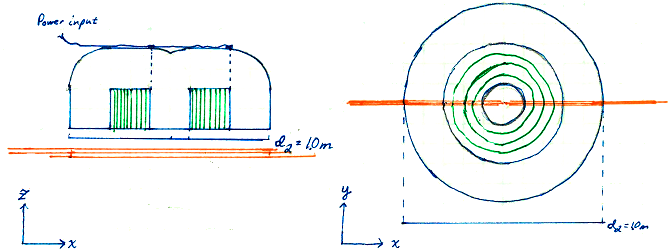
\includegraphics[scale=0.9]{electromagnet.png}
  \caption{Sketch of the head of the electromagnet from a side-on view (left)
  and a top-down view (right)}
\end{figure}

\subsection*{Electromagnet Properties:}
\begin{itemize}
  \item The voltage supplied is always a steady 220V DC
  \item The current can be adjusted from 0-2A by the operator
  \item The ${B(H)}$ dependence in the crane is:
  \[ B(H)=\frac{B_0 H}{H_0 + H} \]
  \item Where the coefficients are approximated as:
    \[B_0=2.2 T\]
    \[H_0=50 A/m\]
  \item The permeability of the core is assumed to be very high
  \item The mass of the magnet itself is 800kg.
  \item The total diameter of the electromagnet is 1m
  \item The coils inside are layers of copper insulated by mica and asbestos,
    the total coil assembly is a toroid with a thickness of 0.2m.
  \item The mean radius of the square toroid core is $R=0.2m$.
\item The surrounding ferromagnetic material is always \emph{at least} a thickness of
    0.2m around the core, except at the base, which is covered with a thin
    steel plate to protect the coils. 
\end{itemize}

\subsection*{Rebar Properties:}
\begin{itemize}
  \item Each rod of rebar is 8kg/m
  \item Each rod of rebar is 10m long
  \item Each rod of rebar has a diameter of 36mm
  \item Rebar comes in bundles of 10
\end{itemize}



\section{Magnetic Field Intensity $\vec{H}$}


\section{Magnetic Flux $\Phi$}
Find the magnetic flux through the electromagnet to the rebar. Assume that a
``bundle'' of rebar is a sheet of 10 rebar rods tied together. \emph{(Hint:
start by finding $S$)}

\sol  To simplify the problem, neglect
the area of the electromagnet that isn't above the rebar rods. Namely, let $S$
be the surface area common between rebar and any one of the segments of
electromagnet. Because the width of the rebar raft is small, this segment can
be approximated as a rectangle:

\[ S \approx 0.2m \cdot (10 \cdot 36mm) = 72mm^2\]




\section{Magnetic Flux Density $\vec{B}$}
Let $N=4000$. The current has been set to $I=1A$ 

\sol
\section{Magnetic Forces}
\sol
\section{B(H) Dependence}
\sol
\section{Magnetic Energy}
\sol
\subsection{What is the force required to lift the rebar?}

\sol First, calculate the force on the rebar due to
gravity:
  \[  F_g = mg \]
Mass of a bundle of rebar:
  \[  m = 10m \cdot 8kg/m \cdot 10 = 800kg\]
  \[  F_g = 800kg \cdot 9.81 m/s = 7.848kN \approx \boxed{7.9kN}\]
\section{Faraday's Law and Inductance}
Once the rebar hauling is completed, the workers decide to use it to move
other items on the construction site. One such item is a ring-shaped piece of
copper pipe with a diameter that is 1m. Unfortunately, the construction
workers forgot that copper is diamagnetic, and assume that the metal ring is
simply stuck. The  confused operator of the crane moves the magnet only inches
away from the ring, such that the $\vec{B}$ field through it is effectively
uniform. When this has no effect, he fiddles with various knobs that have an
unknown purporse, and asks his friend to ``free'' the pipe while he tries to
get the crane to work
``better''. One such button  the frustrated operator presses initializes a
sinusoidal oscillation in the supplied voltage of 60Hz, with the RMS value
being equal to the DC value of the crane in DC mode (220V). The operator's
friend is not wearing any gloves, and has exceptionally sweaty hands.

When the operator's coworker grabs the metal ring, he grabs it such that there
is 1/3 of the circumference of the ring between his two hands
\subsection{ How much current passes through the coworker?}
\subsection{ Will the coworker live?}

\section{Magnetic Fields and the Trajectory of Electrons (Amp\`ere's Law)}
During break, many of the workers are watching TV on an old CRT set.
However, the workers have since continued watching TV instead of returning to
work, and the impatient foreman decides to get their attention by using the
electromagnetic crane.

With the magnetic unit positioned a very short height over the set, the
foreman
fires up the electromagnet as seen in the figure below. Assuming that the TV
is smaller than the magnet (and that the $\vec{B}$ field is approximately
uniform)

\subsection{Describe and/or sketch what the workers see on the screen once the
magnet has stabilized.}
\subsection{The foreman is determined to try and destroy the television. Even
  with the magnet on top of the set and the current at maximum, can he do it?
If so, what current value will destroy the set?}
\sol
  \begin{enumerate}[(a)]
    \item The screen will be distorted and will move to the left because the
      electrons moving in a magnetic field can be thought of as currents. As a
      result, their trajectory will change in response.
    \item At maximum current (2A), the electron will only be deflected into the
      wall of the tube.
\end{enumerate}

\end{document}

